\documentclass[10pt,a4paper]{article}
\usepackage[utf8]{inputenc}
\usepackage[portuges]{babel}
\usepackage{a4wide}
\usepackage{indentfirst}
\usepackage{graphicx}
\usepackage{color}
\usepackage[dvipsnames]{xcolor}

\title{\bf{\textcolor{Mahogany}{Projeto de Laboratórios de Informática III}\\Grupo 41}}
\author{ Ana Ribeiro (A82474) \and Jéssica Lemos (A82061) \and Pedro Pinto (A82535)}
\date{abril de 2018}

\begin{document}

\graphicspath{ {/home/jessica/Desktop/} }
\begin{figure}[t]
    \centering
	\center
\includegraphics[width=4cm]{UM}\\
\end{figure}

\maketitle
\thispagestyle{empty}
\cleardoublepage

\thispagestyle{empty}
\tableofcontents
\cleardoublepage
\pagenumbering{arabic}
\setcounter {page}{1}

\section{Introdução}

Este relatório aborda a implementação de um sistema capaz de processar ficheiros XML que armazenam as várias informações utilizadas pelo Stack Overflow na disciplina de Laboratórios de Informática 3 (LI3), do Mestrado Integrado em Engenharia Informática da Universidade do Minho. Uma vez processada essa informação, pretende-se que seja possivel executar um conjunto de interrogações específicas, apresentadas posteriormente, de forma eficiente.

A substância do relatório centra-se nos seguintes aspectos:
\begin{itemize}
 \item tipo concreto de dados
 \item estruturas de dados usada
 \item modularização funcional
 \item abstração de dados
 \item estratégias seguidas em cada uma das interrogações
 \item estratégias para melhoramento de desempenho
\end{itemize}

\cleardoublepage

\section{Concepção}
\label{sec:solucao}

\subsection{Concepção do problema}

Tendo em conta o problema apresentado, decidimos organizar o nosso trabalho em dois grupos:

\begin{itemize}
 \item Posts
 \item Users
\end{itemize}

Para realizar as queries relativas aos posts é necessário obter do ficheiro \textit{"Posts.xml"} as seguintes informações: o id e o tipo do post e no caso de este ser uma resposta guardar o id da respetiva pergunta, as tags, o seu título, o id do utilizador que o elaborou, a sua data de criação e o número de comentários. Caso o post seja uma pergunta terá de se guardar também o número de respostas. A fim de tornar a resolução das interrogações deste grupo eficientes, é evidente a necessidade de implementar uma estrutura onde seja rápida a procura dos posts de uma dada data. Acrescido a esta preocupação, é indispensável ter o cuidado de organizar os posts de uma data pelo seu id.\\
 \indent  Quanto aos users, é oportuno guardar do ficheiro \textit{"Users.xml"} o id, o nome, a reputação e a informação do seu perfil. Para tornar eficaz a resolução destas queries, é útil estruturar as informações pelo seu id.\\
 \indent Para as tags, é preciso armazenar do ficheiro \textit{"Tags.xml"} o id e o seu nome, ordenadas por este.

\subsection{Concepção da solução}

 Com o objetivo de solucionar todas as interrogações do grupo dos posts de modo eficiente elaboramos uma 
\textit{Hash Table} organizada por datas, em que cada posição contém uma \textit{Árvore Binária Balanceada} com todos os posts dessa data ordenada pelo seu id. A escolha da \textit{Hash Table} deveu-se ao elevado número de interrogações que envolviam intervalos de tempo, para estas tornou-se imperativo evitar percorrer os posts que não tivessem incluídos nesse intervalo. Uma vez reduzida a procura, foi necessário organizar a \textit{Árvore Binária Balanceada} pelo o id do post, dado que a maioria das interrogações se baseiam neste fator.\\
 \indent Para os users optamos por uma \textit{Hash Table} organizada pelos ids dos utilizadores, dado que todas as queries deste grupo se baseiam no id. Houve também a necessidade de associar a cada user uma \textit{MaxHeap} com todos os posts em que participou cujo fator de comparação é a data de criação, para a resolução das interrogações em que é estabelecida uma relação entre o id dos posts e o utilizador ordenados por cronologia inversa.\\
 \indent Tendo em conta que para o grupo das tags a procura se baseia no seu nome definimos uma \textit{Hash Table} disposta por este. Para tal, somamos todas as letras que compunham o seu nome.
Para auxiliar estes dois grupos foi fundamental recorrer a duas \textit{MaxHeaps} para diminuir o tempo de resolução de interregações que envolviam tops. Uma destas incluía os utilizadores estruturados pela sua reputação e a outra engloba os utilizadores ordenados pelo número de posts realizados.
\cleardoublepage

\section{Estrutura de dados}
\label{sec:solucao}
 \noindent O nosso tipo concreto de dados \textit{TCD\_Community} é composta por dez items:
\begin{itemize}
	 \item tamanho de cada tabela de hash
	 \item \textit{Hash Table} que em cada posição contém uma \textit{Árvore Binária Balanceada} dos posts
	 \item \textit{Hash Table} composta pela a informação utilizadores que em cada posição contém uma \textit{MaxHeap} com os ids dos posts em que este participou 
     \item \textit{Hash Table} que possui a informação referente às tags
	 \item \textit{Array} que guarda os ids dos utilizadores com mais posts observados até ao momento
	 \item \textit{Array} que guarda os ids dos utilizadores com maior reputação verificados até ao momento 
	 \item \textit{MaxHeap} que inclui os ids dos utilizadores ordenados pelo número de posts 
	 \item \textit{MaxHeap} que engloba os ids dos utilizadores cujo fator de comparação é a reputação
\end{itemize}

 \noindent {\bf{\textcolor{Emerald}{typedef struct}}} TCD\_community\{\\
	\indent {\bf{\textcolor{Emerald}{int}}} dataSize; \\
	\indent {\bf{\textcolor{Emerald}{int}}} usersSize; \\
	\indent {\bf{\textcolor{Emerald}{int}}} tagsSize;\\
	\indent TreeHashData treeHash;\\
	\indent HashTableUsers hashUser;\\
	\indent HashTableTags hashTag;\\
	\indent {\bf{\textcolor{Emerald}{long}}} *topN;\\
	\indent {\bf{\textcolor{Emerald}{long}}} *topNR;\\
	\indent Heap Top;\\ 
	\indent Heap TopR; \\
\} {\bf{\textcolor{LimeGreen}{TCD\_community}}};	\\

 \noindent {\bf{\textcolor{Emerald}{typedef struct}}} TCD\_community* {\bf{\textcolor{LimeGreen}{TAD\_community}}};\\

O nosso tipo abstracto de dados, \textit{TAD\_Community}, foi declarado no ficheiro .h como sendo um apontador para o nosso tipo concreto de dados. Deste modo, foi possível garantir que a implementação dos dados não se encontra visível para os utilizadores.\\

\subsection{TreeHashData}
\begin{center}
\graphicspath{ {/home/jessica/Desktop/} }
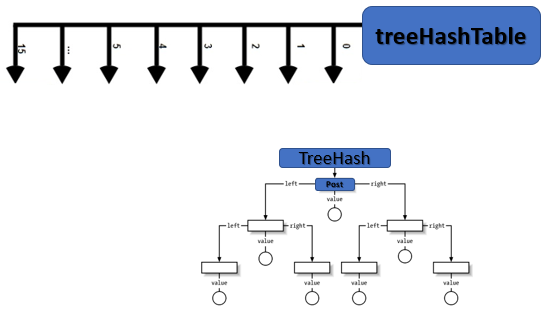
\includegraphics[width=8cm]{Posts}\\
\end{center}

No nodo de cada \textit{Árvore Binária Balanceada} temos as informações necessárias para responder às interrogações referentes ao grupo dos posts.\\

 \noindent {\bf{\textcolor{Emerald}{typedef struct}}} post\{ \\
	\indent {\bf{\textcolor{Emerald}{int}}} postTypeId;\\ 
	\indent {\bf{\textcolor{Emerald}{long}}} parentId; \\
	\indent {\bf{\textcolor{Emerald}{long}}} id; \\
    \indent {\bf{\textcolor{Emerald}{char}}} *tag; \\
	\indent {\bf{\textcolor{Emerald}{char}}} *title; \\
	\indent {\bf{\textcolor{Emerald}{long}}} ownerUserId; \\ 
	\indent Date creationDate;\\
	\indent {\bf{\textcolor{Emerald}{int}}} answerCount; \\
	\indent {\bf{\textcolor{Emerald}{int}}} commentCount; \\
	\indent {\bf{\textcolor{Emerald}{int}}} score; \\
    \indent {\bf{\textcolor{Emerald}{struct}}} post *esq,*dir; \\
\} {\bf{\textcolor{LimeGreen}{Post}}};\\

Cada local da \textit{Hash Table} é constituída pela árvore dos posts. Acrescentamos ainda três variáveis que contam respetivamente: o número de posts tipo resposta, o número de posts tipo pergunta e o número total de posts destes dois tipos.\\

 \noindent {\bf{\textcolor{Emerald}{typedef struct}}} treeHash\{ \\
    \indent {\bf{\textcolor{Emerald}{long}}} contadorR; \\
    \indent {\bf{\textcolor{Emerald}{long}}} contadorP; \\
    \indent {\bf{\textcolor{Emerald}{int}}} numRespostas; \\
    \indent Post* tree; \\
\} {\bf{\textcolor{LimeGreen}{TreeHash}}};\\

 \noindent {\bf{\textcolor{Emerald}{typedef struct}}} treeHash ** {\bf{\textcolor{LimeGreen}{TreeHashData}}};

\subsection{HashTableUsers}

\begin{center}
\graphicspath{ {/home/jessica/Desktop/} }
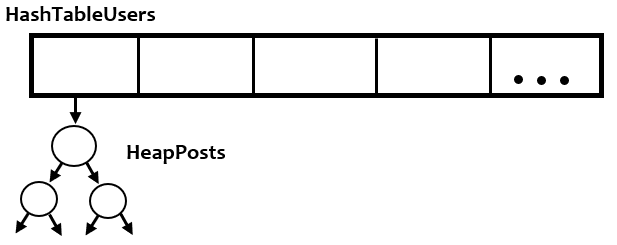
\includegraphics[width=8cm]{Users}\\
\end{center}

Em cada posição da \textit{MaxHeap} existe a data que é o fator de ordenação e o id do utilizador, que é devolvido nas queries em que é utilizada.\\

 \noindent {\bf{\textcolor{Emerald}{typedef struct}}} elemPosts\{\\
    \indent {\bf{\textcolor{Emerald}{long}}} id;  \\
    \indent Date data; \\
\} {\bf{\textcolor{LimeGreen}{elemP}}};\\

 \noindent {\bf{\textcolor{Emerald}{typedef struct}}} heapPosts\{\\
    \indent {\bf{\textcolor{Emerald}{int}}}  size; \\
    \indent {\bf{\textcolor{Emerald}{int}}}   used; \\
    \indent elemP *array;\\
\}* {\bf{\textcolor{LimeGreen}{HeapPosts}}};\\

Em cada lugar da \textit{Hash Table} incluimos as informações necessárias para as interrogações deste grupo e a \textit{MaxHeap} referida anteriormente.\\  

 \noindent {\bf{\textcolor{Emerald}{typedef struct}}} users\{\\
	 \indent {\bf{\textcolor{Emerald}{long}}} ownerUserId; \\
	 \indent {\bf{\textcolor{Emerald}{char}}} *displayName; \\
	 \indent {\bf{\textcolor{Emerald}{int}}} reputation; \\
	 \indent {\bf{\textcolor{Emerald}{int}}} nPosts; \\
	 \indent {\bf{\textcolor{Emerald}{char}}} *aboutMe;\\
	 \indent HeapPosts top10;\\
\} {\bf{\textcolor{LimeGreen}{Users}}};\\

 \noindent {\bf{\textcolor{Emerald}{typedef struct}}} users ** {\bf{\textcolor{LimeGreen}{HashTableUsers}}};

\subsection{HashTableTags}

Em cada lugar da \textit{Hash Table} colocamos as informações necessárias para a resolução de uma das queries. \\  

 \noindent {\bf{\textcolor{Emerald}{typedef struct}}} tags\{\\
	\indent {\bf{\textcolor{Emerald}{long}}} id; \\
	\indent {\bf{\textcolor{Emerald}{char}}} *tagName;\\
\} {\bf{\textcolor{LimeGreen}{Tags}}};\\

\noindent {\bf{\textcolor{Emerald}{typedef struct}}}  tags **{\bf{\textcolor{LimeGreen}{HashTableTags}}};

\subsection{Heap}

Em cada posição da \textit{MaxHeap} encontra-se o uma variável que é o fator de ordenação, que depende do contexto em que é aplicada e o id do utilizador, que é devolvido nas queries em que é usada.\\

 \noindent {\bf{\textcolor{Emerald}{typedef struct}}} elemento\{\\
    \indent {\bf{\textcolor{Emerald}{long}}} id; \\
    \indent {\bf{\textcolor{Emerald}{int}}} count;\\
\} {\bf{\textcolor{LimeGreen}{elem}}};\\

 \noindent {\bf{\textcolor{Emerald}{typedef struct}}} heap{\\
    \indent {\bf{\textcolor{Emerald}{int}}}   size; \\
    \indent {\bf{\textcolor{Emerald}{int}}}  used; \\
    \indent elem *array;\\
\}* {\bf{\textcolor{LimeGreen}{Heap}}};\\

\section{Interrogações}
\label{sec:solucao}

\subsection{Init}
Na query init simplesmente alocamos espaço para a estrutura \textit{TAD\_Community}, inicializamos as \textit{Hash Tables}, as \textit{MaxHeap} e os \textit{Arrays}, dado que é no load que iniciamos as estruturas que constituem a \textit{TAD\_Community} pois apenas temos acesso aos tamanhos necessários no \textit{parse}.

\subsection{Load}
Esta interrogação é a mais demorada visto que é responsável por processar a informação dos ficheiros e armazená-la na nossa estrutura. Tendo em conta a variedade dos requesitos apresentados nas queries, optamos por estruturas mais complexas que se refletiram no tempo de load mas que se irá expressar numa maior efeciência na resolução das interrogações.

\subsection{Info\_from\_post}
Começamos por procurar o post na \textit{TreeHashData} e caso este seja do tipo pergunta retiramos-lhe o título e id do utilizador. Com o id acedemos à estrutura dos users e obtemos o nome do utilizador. Na eventualidade do post ser do tipo resposta retiramos o id da pergunta a que corresponde e efetuamos o proceso anterior para este.

\subsection{Top\_most\_active}
Recorrendo à \textit{MaxHeap} que se encontra ordenada pelo número de posts de cada utilizador, extraimos os N ids pedidos, guardamos no \textit{Array} que está na \textit{TAD\_Community} e criamos a lista necessária para devolver. No caso do array já ter algum id, o que ocorre quando a query é invocada mais do que uma vez, aproveitamos os ids já existentes no array e caso necessário extraimos o que falta para completar o requerido.

\subsection{Total\_posts}
Para esta query percorremos a \textit{TreeHashData} e no caso de a data pertencer ao intervalo de tempo pertendido, somamos aos contadores do número de respostas e número de perguntas respetivamente, e de seguida criamos o par esperado com essa informação.

\subsection{Questions\_with\_tag}
Iniciamos por percorrer a \textit{TreeHashData} e na hipótese de a data estar contida no intervalo de tempo desejado, vamos a todos os nodos da árvore e na eventualidade de o post ser do tipo pergunta, verificamos se a tag dada se encontra nas tags do post. Em caso afirmativo, guardamos o id num \textit{array} ordenado por datas que no final será transferido para a lista solicitada.

\subsection{Get\_user\_info}
Nesta interrogação acedemos à posição onde se encontra o utilizador pretendido na \textit{HashTableUsers} e obtemos a informação do
seu perfil e extraimos da \textit{MaxHeap} integrante os seus dez últimos posts.

\subsection{Most\_voted\_answers}
Começamos por percorrer a \textit{TreeHashData} e na possibilidade de a data se enquadar no intervalo de tempo pedido, acedemos a todos os nodos da árvore e caso seja do tipo resposta inserimos o score e o id em dois \textit{arrays} de tamanho solicidado na query  e com fator de comparação o score. Desta forma, apenas são inseridos elementos que potencialmente poderão integrar-se no top N pretendido.

\subsection{Most\_answered\_questions}
Para esta query passamos por todas as posições da \textit{TreeHashData} e no caso da data se encontrar no intervalo requerido, percorremos a estrutura dos posts calculando a chave para a \textit{HashTableQuery7} onde inserimos uma flag para o caso do post ser do tipo pergunta e um contador para incrementar no caso do tipo resposta. De seguida, extraimos da \textit{MaxHeap} criada com os elementos da \textit{Hash Table} com flag a 1 (indica que o post é tipo pergunta) e o número de respostas feitas a esse post neste mesmo intervalo. Por fim, devolvemos os ids dos posts ordenados por cronologia inversa.\\
\indent De modo a tornar mais eficiente a resolução desta query decidimos implementar uma \textit{Hash Table} em que em cada posição guardamos o id do post tipo pergunta, bem como uma flag indicando se este se encontra neste intervalo de tempo e um contador com o número de posts tipo resposta. Desta forma, a inserção e posteriormente a procura na \textit{Hash Table} para a inserção na \textit{MaxHeap} será muito mais rápida e eficaz do que seria com a utilização, por exemplo, de \textit{arrays}, que para tamanhos consideravelmente grandes torna-se bastante ineficiente.\\

\noindent {\bf{\textcolor{Emerald}{typedef struct}}} query7\{\\
    \indent {\bf{\textcolor{Emerald}{long}}} id;\\
    \indent {\bf{\textcolor{Emerald}{int}}} flag;\\
    \indent {\bf{\textcolor{Emerald}{int}}} contador;\\
\} {\bf{\textcolor{LimeGreen}{Query7}}};\\

\noindent {\bf{\textcolor{Emerald}{typedef struct}}} query7 ** {\bf{\textcolor{LimeGreen}{HashTableQuery7}}};

\subsection{Contains\_word} 
Passamos por todos os Posts existentes e na eventualidade de ser do tipo pergunta verificamos se a palavra dada se encontra no título. Em caso afirmativo, inserimos em dois \textit{arrays} com o tamanho solicitado, o id e a data, ordenados por esta.

\subsection{Both\_participated} 
Começamos por aceder às posições da \textit{HashTableUsers} dos utilizadores solicitados e retiramos as respetivas \textit{MaxHeaps}. Extraimos os ids da maior das \textit{MaxHeaps} para um \textit{array}, mas caso o post a extrair seja do tipo resposta, guardamos o id da pergunta correspondente. De seguida, removemos os elementos da outra das \textit{MaxHeaps} e verificamos se é do tipo pergunta ou tipo resposta. Na eventualide de ser do tipo pergunta, verificamos se o id deste se encontra no \textit{array} criado anteriormente. Caso contrário, retiramos o parentId e utilizamos este como fator de comparação.

\subsection{Better\_answer} 
Nesta query, percorremos a \textit{TreeHashData} e os nodos da \textit{Árvore Binária Balanceada} até encontrar o post requerido e retiramos o número de respostas existente. Depois voltamos a percorrer a \textit{TreeHashData} a partir dessa posição e sempre que encontramos um resposta ao post vamos buscar as informações necessárias para obter a média ponderada e decrementamos ao número de respostas existentes, pois deste modo evitamos continuar a percorrer a estrutura quando já não houverem mais respostas à pergunta. Sempre que encontramos uma média maior do que a guardada até ao momento, substituimos esse valor e atualizamos o id. Na possibilidade de chegarmos ao fim da hash e ainda existirem respostas retomamos a procura desde o início. No caso de o id dado corresponder a um post resposta o número de respostas será zero e não efetuará qualquer cálculo. 

\subsection{Most\_used\_rep} 
Iniciamos por preencher o \textit{array} com os ids dos utilizadores com melhor reputação que faltam para obter o top N pretendido e transferimo-los para a \textit{HashTableTopN}, pois a procura de um utilizador num \textit{array} consideravelmente grande seria muito lenta. De seguida percorremos a \textit{TreeHashData} e se a data da posição pertencer ao intervalo de tempo, acedemos aos nodos da árvore e para cada um verificamos se o utilizador está incluido no top N estabelecido anteriormente. Caso tal se suceda, para todas as tags desse post vamos verificar se o seu id já se encontra na \textit{HashTableQuery11} e caso esteja incrementamos o número de vezes que esta ocorre. Caso contrário, vamos procurá-la à estrutura das tags e inserimos o seu id na nossa \textit{Hash Table}. Posteriormente os elementos da \textit{Hash Table} são inseridos numa \textit{MaxHeap} de modo a obtermos as N tags mais usadas pelos N utilizadores com melhor reputação.\\
\indent Na resolução desta query seguimos o raciocínio da interrogação 7, sendo que nesta \textit{Hash Table} decimos em cada posição guardar o id da tag de modo a não procurar a mesma na \textit{HashTableTags} repetidamente, a própria e um contador com o número de vezes que esta é utilizada. Como já referido, a inserção e posteriormente a procura será muito mais rápida e eficaz.\\

\noindent {\bf{\textcolor{Emerald}{typedef struct}}} query11\{\\
    \indent {\bf{\textcolor{Emerald}{long}}}} id;\\
    \indent {\bf{\textcolor{Emerald}{char*}}} tag;\\
    \indent {\bf{\textcolor{Emerald}{long}}} contador;\\
\} {\bf{\textcolor{LimeGreen}{Query11}}};\\

\noindent {\bf{\textcolor{Emerald}{typedef struct}}} query11 ** {\bf{\textcolor{LimeGreen}{HashTableQuery11}}};

\subsection{Clean} 
Percorremos todas as estruturas criadas libertando as informações para o qual foi alocada memória. Tendo ainda o cuidado de libertar os arrays.

\section{Modularidade}
\label{sec:solucao}
Dada a dimensão do projeto, foi imperativo organizá-lo de modo a torná-lo monitorizável e legível. Para tal, optamos por dividi-lo em módulos, sendo os fundamentais o \textit{parse} e a \textit{struct}. No \textit{parse} é realizado o \textit{parsing} dos ficheiros XML utilizando a biblioteca \textit{libxml}. Na \textit{struct} inicializamos, carregamos e libertamos as estruturas com os dados provenientes do  \textit{parse}.\\
\indent Quanto às interrogações estruturamo-las em dois grupos: users e posts. Sendo que as estruturas auxiliares encontram-se num novo módulo, a \textit{auxiliary}.

\section{Melhoramento de desempenho}
\label{sec:solucao}
As \textit{flags} do tipo \textit{-O} definem o nível de otimização do compilador. Neste caso, optamos por utilizar a \textit{flag -O3} de modo a melhorar o desempenho do código resultando num melhor tempo de execução. Testamos também a \textit{flag -O2} para comparar o tempo de execução com as diferentes \textit{flags} e verificamos que com a \textit{flag -O3} o desempenho era consideravelmente melhor.

\section{Conclusão}
\label{sec:conclusao}
Neste trabalho foi notória a importância da escolha das estruturas a utilizar, uma vez que estas têm influência direta no desempenho das interrogações requeridas. Para desenvolver este projeto optamos por estruturas mais complexas que demoram mais tempo a serem carregadas, mas que permitem um melhor tempo de execução das queries. O facto de cada interrogação poder ser invocada mais do que uma vez contribuiu para esta decisão.\\
\indent Com o objetivo de melhorar o tempo de load, ao longo do trabalho pensamos em alterar as estruturas. No entanto, na resolução das queries verificamos que uma estrutura menos bem conseguida tinha um impacto negativo no seu desempanho.\\
\indent Em última instância, consideramos que os nossos objetivos neste projeto foram alcançados, contudo ainda podiam ser melhorados alguns aspetos.

\end{document}
\grid
\grid
\grid
